Dieses Projekt verwenden gängige Technologien, welches die Entwicklung vereinfachen und die Integration mit anderen Systemen ermöglichen. Im folgenden werden die wesentlichen T. erklärt.

\section{C\#}
C\# (gesprochen „C-Sharp“) ist eine objektorientierte Programmiersprache, die im Auftrag von Microsoft entwickelt und 2000 veröffentlicht wurde.
Die Sprache ist grundsätzlich plattformunabhängig und wurde für die Softwareplattform .NET entwickelt.
Auf GitHub gehört sie zu den fünf am meisten verwendeten Programmiersprachen.\cite{ms-csharp}

Die Einsatzbereiche dieser Sprache sind nahezu Grenzenlos.
Schon seit Veröffentlichung entstanden Projekte in den Bereichen Webseiten, Entwicklerwerkzeuge und Kompilierer.
Durch diese einfach, moderne und flexible Sprache qualifiziert sie sich auch für dieses Projekt.
Der Zusammenschluss von C und C++ brachte diese Eigenschaften herbei und macht es somit selbst Java Entwicklern einfach, die Sprache zu verwenden.\cite{dev-csharp}

\section{HTTP}
HTTP steht für „Hypertext Transfer Protocol“ und ist das Kommunikationsprotokoll im World Wide Web (WWW).
Es ist für das Abrufen von statischen Inhalten, wie HTML-Dokumenten, vorgesehen und bildet somit die Grundlage für jeden Datenaustausch im Web als Client-Server-Protokoll.
In der Regel werden Anfragen an den Server über einen Browser gestellt, der ebenso die Antwort des Servers empfängt und darstellt.

Das  in den 1990er Entwickelte Protokoll ist erweiterbar und kann mittels TLS Verschlüsselt werden. Es lässt sich inder Anwendungsschicht im ISO/OSI-Referenzmodell einordnen.
HTTP ist zustandslos, da es keine Verbindung zwischen zwei Anfragen gibt, die nacheinander auf der selben Verbindung ausgeführt werden, kann aber mittels HTTP-Cookies für zustandshafte Sitzungen Verwendung finden.\cite{mdn-http}

HTTP-Antworten enthalten die Version des Protokolls, Header, den Statuscode der angibt, ob die Anfrage erfolgreich war (wie in Abbildung \vref{http-response} gezeigt), eine Status-Nachricht und den Körper der Nachricht mit dem angeforderten Inhalt.
HTTP-Header ermöglichen Client und Server den Austausch zusätzlicher Informationen, so z.B. für die Authentifizierung des Clients am Server, für das verwendete Caching (Pufferspeichern) oder gespeicherte Cookies.\cite{mdn-http-header}

\begin{figure}[ht]
	\centering
	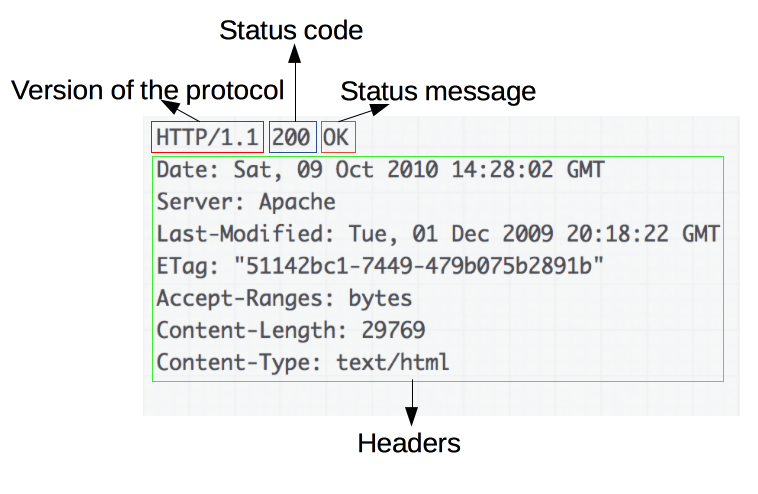
\includegraphics[width=0.7\linewidth]{http_response.png}
	\caption{Beispiel einer HTTP-Antwort}
	\label{http-response}
\end{figure}

\section{IDE}
%bearbeiten
Für eine effiziente Arbeitsweise benötige ich Programme, welche mir beim Schreiben des Quelltextes helfen und diesen für mich kompilieren, damit am Ende eine ausführbare Anwendung bereitsteht. Auch hier greife ich wieder auf eine mir bereits bekannte Lösung von Microsoft zurück: Microsoft Visual Studio 2022. Das Programm bietet hilfreiche Funktionen wie das automatische Installieren von Paketen, das farbige Markieren von Quelltexten für eine bessere Lesbarkeit und einen Kompilierer, der C-Sharp versteht. Die IDE gibt mir außerdem Möglichkeiten in meine Anwendung während der Laufzeit hereinzuschauen, um Fehler schneller finden zu können sowie die Korrektheit der Vorgänge zu überprüfen.

\section{Git}
Git ist ein ausgereiftes, aktiv gepflegtes Open-Source-Projekt, das ursprünglich 2005 von Linus Torvalds, entwickelt wurde.
Eine erstaunliche Anzahl von Softwareprojekten verlässt sich auf Git für die Versionskontrolle, einschließlich kommerzieller Projekte sowie Open Source.
Im Gegensatz anderer Versionskontrollsoftware lässt sich Git bei der Versionshistorie des Dateibaums nicht von den Namen der Dateien täuschen, stattdessen konzentriert sich Git auf den Dateiinhalt selbst.
Somit gehört es mit zu den Leistungsstärksten seiner Art.
Die Integriergerät des Quellcodes war bei der Entwicklung die höchste Priorität. Der SHA1 Algorithmus wird für die Sicherung der Verzeichnissen verwendet. So wird der Verlauf vor Änderungen beschützt.

Git zeichnet sich ebenso durch seine Flexibilität aus: es Unterstützt verschiedene Arten von Entwicklerworkflows, die nichtlinear sind. Es eignet sich somit für alle Größen von Projekten.\cite{git}
Durch die Einteilung von Git in drei Arbeitsbereiche können Änderungen flexibel angebracht werden.

Im Arbeitsverzeichnis (Working Directory) liegen alle Projektdateien zur Bearbeitung oder Benutzung.
Änderungen an diesen Dateien werden im Entwicklungsbereich (Staging Area) erfasst und aufbewahrt.
Um diese Änderungen zu veröffentlichen, muss ein Commit (Beitrag) erzeugt werden, welcher die Informationen der Änderungen trägt.
Diese können dann im Versionsverlauf des Git Verzeichnisses gespeichert werden. Abbildung \vref{git-sections} stellt diese Beziehungen dar.

\begin{figure}[ht]
	\centering
	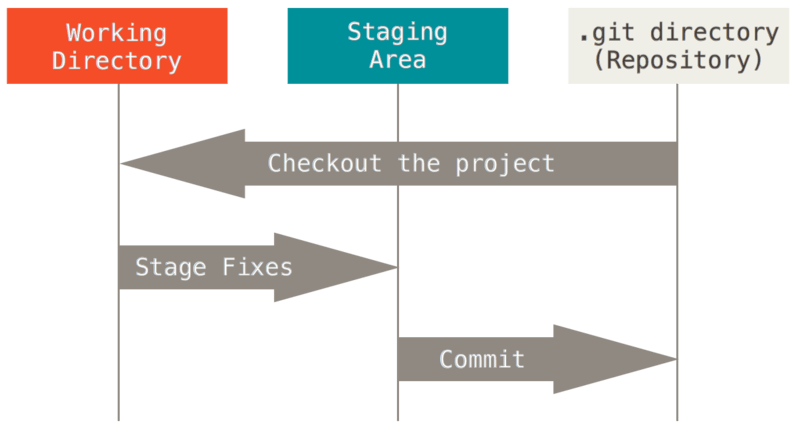
\includegraphics[width=0.8\linewidth]{git-sections.png}
	\caption{Arbeitsverzeichnis, Entwicklungsbereich, Git Verzeichnis}
	\label{git-sections}
\end{figure}

\section{SQLite}
Das relationale Datenbank-Management-System (DBMS) ist eine leichtgewichtige Lösung, die ohne Server auskommt, für eine schnelle Datenbankanbindung. Die Open-Source-Software kann in Anwendungen integriert werden, um Speicherung von Daten ohne separaten Datenbankserver zu ermöglichen. SQLite wurde in C geschrieben und ist mit vielen Betriebssystem wie Windows, Linux, MacOS, Android und iOS. Unterstützt werden grundlegende SQL-Operationen wie INSERT, UPDATE; SELECT und DELETE. Abfragen mit Aggregatfunktionen, Unterabfragen und Joins sind ebenso möglich. Durch die ACID-Konformität ist Zuverlässigkeit und Robustheit gewährleistet. Der Funtkionsumfang ist gegenüber MySQL sehr eingeschränkt. Diese Einschränkung haben jedoch keinen negativen Einfluss auf das Projekt.

\section{Kanban}
Kandban ist ein Arbeitsmodus, indem ein Projekt in kleine Arbeitspakete zerlegt wird und diese mithilfe eines Boards geplant werden können.
Das Board besteht aus Spalten TODO, In Progress, Done als einfachste Form.
Ein Vorteil dieser Arbeitsweise ist, einen direkten überblicke über getane und geplante Arbeit zu erhalten.
Du durch einzelne Spalten könne zusätzlich priorisierte Gruppen erstellt werden.
Beim Kollaborativen Arbeiten werden die Tickets, die in Bearbeitung sind, einer Verantwortlichen Person zugewiesen.
Um den Erfolg einer Arbeit in Kanban zu messen, verwendet man zwei wesentliche Metriken: die Zykluszeit, welche die benötige Zeit für eine Aufgabe misst und den Durchsatz, der die Anzahl der abgeschlossenen Daten für eine bestimmte Zeiteinheit zurückgibt. \cite{kanban}

Eine weitere Darstellungsform des Erfolgs ist das kumulatives Flussdiagramm (CFD). Es veranschaulicht die Anzahl der Elemente (Vertikale Achse) im Laufe der Zeit (Horizontale Achse). Die Zustände der Bereiche werden mir Farben gekennzeichnet, wie Abbildung \vref{cfd} zeigt. Sind die Verläufe der Bereiche nahezu parallel, wurde der Zeitplan eingehalten.

\begin{figure}[ht]
	\centering
	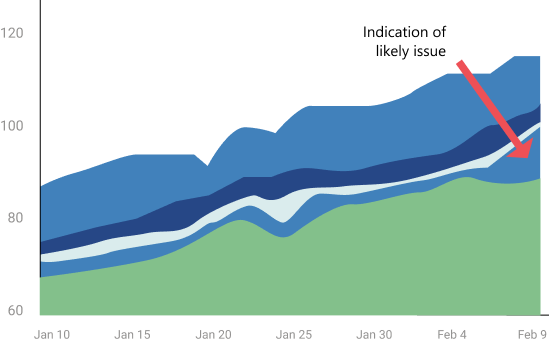
\includegraphics[width=0.7\linewidth]{kanban-cumulative-flow-2.png}
	\caption{Beispiel eines CFD mit Verschiebung im Zeitplan}
	\label{cfd}
\end{figure}

\section{Testing}
Um sicherzustellen, das die Software den gestellten Anforderungen entspricht, müssen zentrale Bestandteile dieser durch Tests abgesichert werden.
Es gibt verschiedene Arten von Test, von denen die wichtigsten Unit-Test sind.
Hierbei handelt es sich um de Prüfung isolierter Softwarebestandteile, die gegen vordefinierte Daten geprüft werden.
Zu beachten ist, das Tests keine Fehlerfreiheit garantieren können, jedoch insbesondere die Software gegen Fehler durch Erweiterungen robust machen.\cite{ms-testing}

Andere Arten von Softwaretest sind Integration- und Smoke-Test, welche als Blackboxtest zusammengefasst werden können.
Integrationstests überprüfen die einzelnen Module einer Software auf ihre Zusammenarbeit mit anderen.
So können z.B. Datenbankanbindungen und Microservices auf ihre Funktionalität geprüft werden.\cite{atlassian-testing}

Allgemein sollen Tests Sicherheit, Produktqualität und Kostenersparnisse sichern.
Wenn ein defekt in der Software nicht Zeitnah erkannt wird, steigt der Suchaufwand nach des Auslösers in komplexen Projekten enorm.
Werden Fehler in der frühen Entwicklungsphase behoben, werden so die Kosten für die weiteren Entwicklung niedriger gehalten.
Sicherheitslücken die noch vor der Veröffentlichung einer Version geschlossen werden, bieten Angreifern keine Möglichkeit eine Software zu missbrauchen.
Nebenbei sei auch erwähnt, dass eine fehlerfreie Software mehr Kundenzufriedenheit bedeutet.\cite{stm-testing}